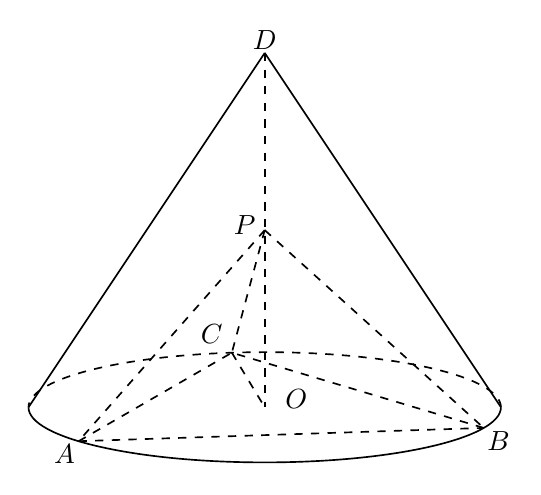
\begin{tikzpicture}[line width=0.6pt, font=\normalsize]
% Cone D with base centre O, inscribed equilateral ABC, P on DO
\coordinate (D) at (0,4.5);
\coordinate (O) at (0,0);
\coordinate (P) at (0,2.25);
\coordinate (A) at (-2.364032261,-0.4309630327);
\coordinate (B) at (2.781551564,-0.2622246154);
\coordinate (C) at (-0.4175193029,0.6931876481);
% cone outline solid
\draw (D) -- (-3,0);
\draw (D) -- (3,0);
% base ellipse: front solid, back dashed
\draw (-3.0,0) arc (180:360:3.0 and 0.7);
\draw[dashed] (3.0,0) arc (0:180:3.0 and 0.7);
% axis and interior dashed
\draw[dashed] (D) -- (O);

\draw[dashed] (P) -- (A);
\draw[dashed] (P) -- (B);
\draw[dashed] (P) -- (C);
\draw[dashed] (A) -- (B);


\draw[dashed] (C) -- (O);
\draw[dashed] (A) -- (C);
\draw[dashed] (B) -- (C);
% labels with clearance
\node[inner sep=1pt,above] at (D) {$D$};
\node[inner sep=1pt,left,xshift=-2.00bp,yshift=2.00bp] at (P) {$P$};
\node[inner sep=2pt,right] at (.18,.10) {$O$};
\node[inner sep=1pt,below left] at (A) {$A$};
\node[inner sep=1pt,below right] at (B) {$B$};
\node[inner sep=3pt,above left] at (C) {$C$};
\end{tikzpicture}
